\documentclass[a4paper, 11pt]{article}
\usepackage[polish]{babel}
\usepackage[MeX]{polski}
\usepackage[utf8]{inputenc}
\usepackage[T1]{fontenc}
%\usepackage{times}
\usepackage{graphicx,wrapfig}
%\usepackage{anysize}
%\usepackage{tikz}
%\usetikzlibrary{calc,through,backgrounds,positioning}
\usepackage{anysize}
\usepackage{float}
\usepackage{adjustbox}
%\usepackage{stmaryrd}
%\usepackage{amssymb}
%\usepackage{amsthm}
%\marginsize{3cm}{3cm}{3cm}{3cm}
%\usepackage{amsmath}
%\usepackage{color}
%\usepackage{listings}
%\usepackage{enumerate}
%\lstloadlanguages{Ada,C++}
\usepackage{enumitem}



\begin{document}	
	% \noindent -  w tym akapicie nie bedzie wciecia
	% \ indent - to jest aut., ale powoduje ze jest wciecie
	% \begin{flushleft}, flushright, center - wyrownianie akapitu
	% \textbf{pogrubiany tekst}
	% \textit{kursywa} 
	% 					STRONY 
	%  http://www.codecogs.com/latex/eqneditor.php 
	%  http://www.matematyka.pl/latex.htm
	% 
	\begin{titlepage}
		
		
		
		\newcommand{\HRule}{\rule{\linewidth}{0.5mm}} % Defines a new command for the horizontal lines, change thickness here
		
		\center % Center everything on the page
		
		%----------------------------------------------------------------------------------------
		%	HEADING SECTIONS
		%----------------------------------------------------------------------------------------
		
		\textsc{\LARGE Akademia Górniczo-Hutnicza im. Stanisława Staszica}\\ % Name of your university/college
		\textsc{\Large Wydział Elektrotechniki, Automatyki, Informatyki i Inżynierii Biomedycznej}\\[0.5cm] % Major heading such as course name
		\textsc{\Large Kraków}\\[0.5cm] % Major heading such as course name
		\hfill
\includegraphics[scale=0.5]{Img/logoAgh.jpg}\hspace*{\fill}
		
		\begin{center}
				\begin{figure}[H]%[!htb]
				%
\includegraphics[scale=0.5]{logoAgh.jpg}
				\end{figure}
	    \end{center}
		\textsc{\large Inżynieria Oprogramowania}\\%[0.5cm] 
		\textsc{\large Informatyka, III rok}\\[0.5cm] % Minor heading such as course title
		
		%----------------------------------------------------------------------------------------
		%	TITLE SECTION
		%----------------------------------------------------------------------------------------
		
		\HRule \\[0.4cm]
		{\fontsize{38}{50}\selectfont Hotel}
		%	{ \Huge \bfseries} Osadnicy z Catan - Gra sieciowa\\[0.3cm] % Title of your document
		\HRule \\[1.5cm]
		
		%----------------------------------------------------------------------------------------
		%	AUTHOR SECTION
		%----------------------------------------------------------------------------------------
	
		% If you don't want a supervisor, uncomment the two lines below and remove the section above
		\Large \emph{Autorzy:}\\
		Sebastian \textsc{Katszer}\\
		Katarzyna \textsc{Kosiak}\\[1cm]\ % Your name
			\Large \emph{Prowadzący:}\\
			dr inż. Radosław \textsc{Klimek}\\[2cm]\ % Your name
		
		
		%----------------------------------------------------------------------------------------
		%	DATE SECTION
		%----------------------------------------------------------------------------------------
		
		{\large \today}\\[3cm] % Date, change the \today to a set date if you want to be precise
		
		%----------------------------------------------------------------------------------------
		%	LOGO SECTION
		%----------------------------------------------------------------------------------------
		
		%\includegraphics{Logo}\\[1cm] % Include a department/university logo - this will require the graphicx package
		
		%----------------------------------------------------------------------------------------
		
		\vfill % Fill the rest of the page with whitespace
		
	\end{titlepage}
	
	%SPIS TRESI
	%
	%
	%
	%
	%
	%
	%
	%
	%
	
	\tableofcontents
	\vfill
	\newpage	%\pagebreak
	
	%SEKCJE
	%opis zagadnienia, temat, problem, dlaczego chcemy to rozwiązacyać metodą ewolucyjnę
	%jakie są metody rozwiącania problemu, przegląd literatury,
	%proponowane rozwiązania (spójność)
	%czym się inspierowałyśmy
	%
	%
	%
	
	%\setlength{\parskip}{1ex plus 0.5ex minus 0.2ex}
	
	%\section{Wstęp}
	%\indent
	
	%Niniejszy dokument stanowi dokumentację projektu ``Hotel'' z przedmiotu Inżynieria Oprogramowania na trzecim roku kierunku Informatyka, na Wydziale Elektrotechniki, Automatyki, Informatyki i Inżynierii Biomedycznej.
	
	\section{Streszczenie systemu}
		\indent
		
	
	Projekt ten modeluje działanie niewielkiego hotelu.\\ \indent
	Hotel ten dysponować będzie pokojami dwu-, trzy- i czteroosobowymi w ilości równiej pięć na każdy typ z możliwością ich rezerwacji na okres minimum doby (osobiście w recepcji, przez telefon lub poprzez stronę internetową). Dostępne są trzy opcje płatności: internetowa, gotówką lub kartą, przy czym rodzaj płatności trzeba podać podczas rezerwacji pokoju, a po jej dokonaniu otrzymuje się potwierdzenie dokonania wpłaty w wybranej formie: rachunek lub fakturę. \\ \indent
	Oprócz procesu przygotowawczego pokoju przed przybyciem klienta, codziennie pokoje są sprzątane na prośbę klienta w godzinach 10:00-12:00.  \\ \indent
	Klient może zamówić posiłki do pokoju, które przygotowywane są przez firmę cateringową i dostarczane przez obsługę hotelową. Klient może zamówić budzenie i taksówkę przez recepcję.	Po zakończeniu pobytu klient może ocenić zadowolenie z usług hotelu poprzez wypełnienie formularza.  \\ \indent
	Po spędzeniu w hotelu sumarycznie dwóch tygodni klient może ubiegać się o kartę stałego klienta uprawniającą do 15 \% zniżki.  \\ \indent
	Niezbędne do funkcjonowania hotelu produkty zamawiane są przez kierownika w hurtowni. Reklama będzie realizowana przez wynajętą agencję. \\
		
	\section{Lista obiektów}	
	
	\begin{itemize}
			\item Pracownicy hotelu:
			
			\begin{itemize}
				\item Kierownik - prowadzi hotel, akceptuje i modyfikuje listę zamówień z hurtowni,
				
				\item Recepcjonista - obsługuje klientów przy rezerwacjach, daje i odbiera dostęp do pokoju klientom, informuje portiera o potrzebie przeniesienia bagaży, na prośbę klienta: budzi go o określonej godzinie, zamawia taksówkę,
				
				\item Pokojowy - przygotowuje pokój przed przybyciem klienta, na prośbę klienta, sprząta pokój, przynosi posiłki, uzupełnia listę zamówień o brakujące środki czystości,
				
				\item Portier - nosi bagaże klientów, udziela informacji klientom o topografii hotelu.
				
			\end{itemize}
		
		\item Pozostali:
		
		\begin{itemize}
			\item Klient - osoba rezerwująca pokój i korzystająca z niego w określonym przez rezerwację czasie,
			
			\item Agencja księgowa - zajmuje się dokumentowaniem spraw finansowych hotelu zgodnie z obowiązującym prawem,
			
			\item Firma cateringowa - realizuje zamówienia klienta, które są przekazywane przez obsługę hotelową,
			
			\item Agencja reklamowa - firma, która zarządza kampanią reklamową hotelu,
			\item Hurtownia - dostarcza produktu, które są potrzebne w hotelu,
			
			\item Strona internetowa - umożliwia rezerwację pokoju przez Internet.
				\vfill	
		\end{itemize}
		
		
		
		
	\end{itemize}
	
	
	\section{Lista zdarzeń}
	
	
	\indent
	\begin{itemize}
		
		\item Klient rejestruje swój pobyt
		\item Klient przybywa i realizuje rezerwację
		\item Klient zamawia sprzątanie pokoju, posiłek, budzenie lub taksówkę,
		\item Klient zdaje pokój w recepcji
		\item Klient dokonuje oceny świadczonych usług w recepcji
		\item Klient dokonuje płatności: gotówką, kartą, internetowo
		\item Hurtownia dostarcza zamówionych przez kierownika produktów
		\item Agencja reklamowa dostarcza hotelowi swoje usługi
		\item Firma cateringowa wydaje polecone zamówienia
		\\
	\end{itemize}
	

	
	\section{Diagram kontekstowy}
	\indent
		\\
	\begin{figure}[H]%[!htb]
			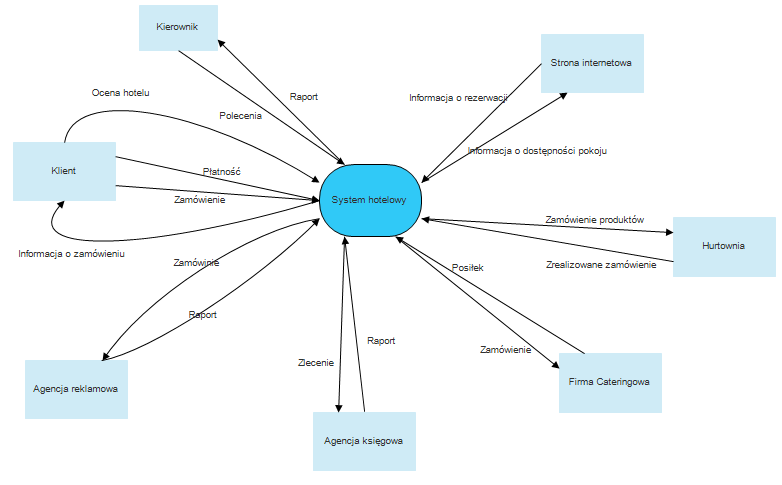
\includegraphics[scale=0.8]{Img/kontekstowy.png}\caption{Diagram kontekstowy}
	\end{figure}


	\vfill		
	\section{Diagramy DFD}
	\indent
	\subsection{poziom 0}
	\indent
	\begin{figure}[H]%[!htb]
			\center
			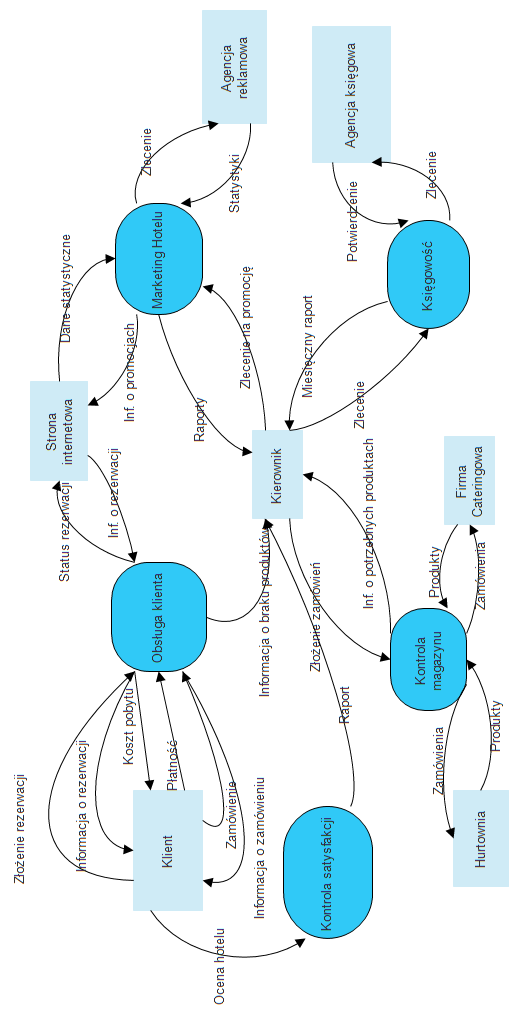
\includegraphics[scale=0.7]{Img/DFDpoziom0.png}\caption{Diagram DFD - poziom 0.}
	\end{figure}

	
	\subsection{poziom 1}
	\indent
	\begin{figure}[H]%[!htb]
			\center
			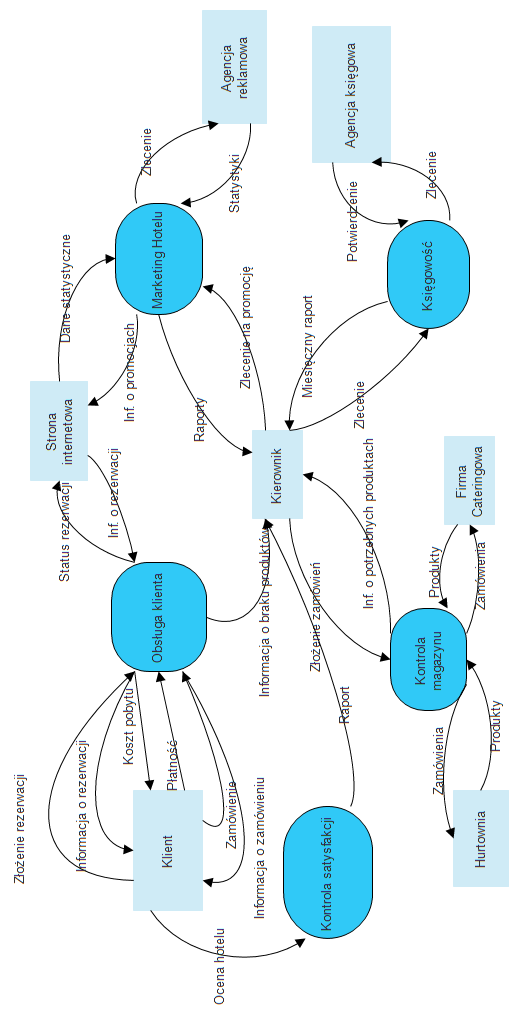
\includegraphics[scale=0.7]{Img/DFDpoziom0.png}
			\caption{Diagram DFD - proces 1.}
	\end{figure}	
	\begin{figure}[H]%[!htb]
			\center
			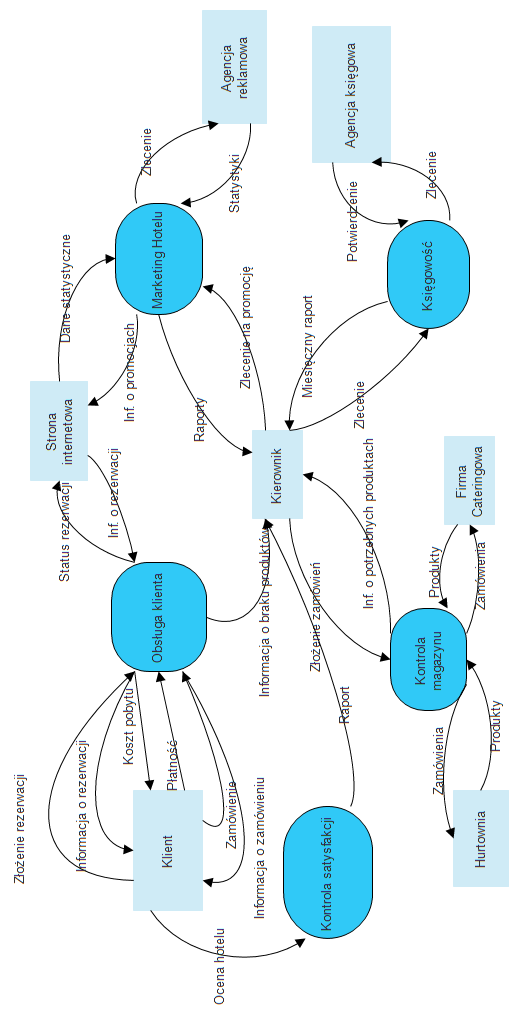
\includegraphics[scale=0.7]{Img/DFDpoziom0.png}
			\caption{Diagram DFD - proces 2.}
	\end{figure}
	\begin{figure}[H]%[!htb]
			\center
			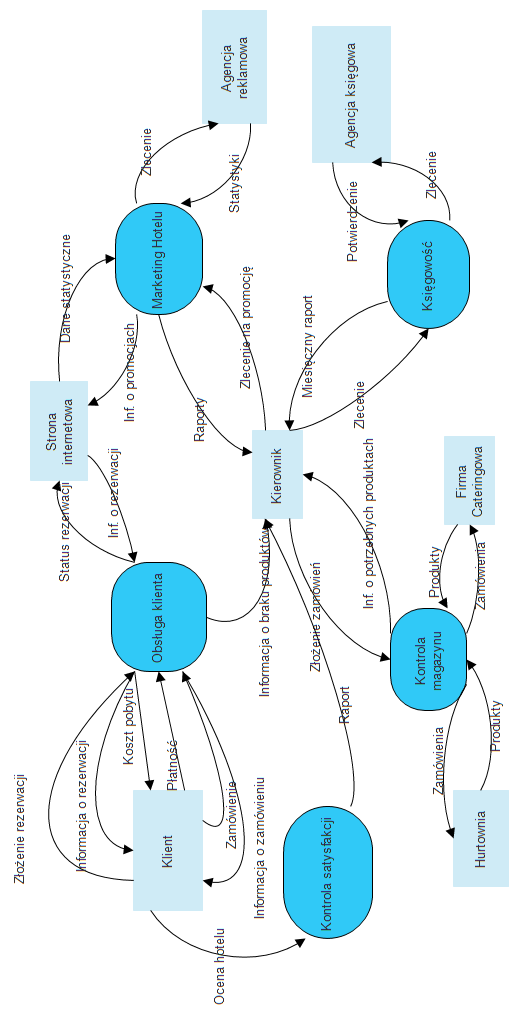
\includegraphics[scale=0.7]{Img/DFDpoziom0.png}
			\caption{Diagram DFD - proces 3.}
	\end{figure}
	\begin{figure}[H]%[!htb]
			\center
			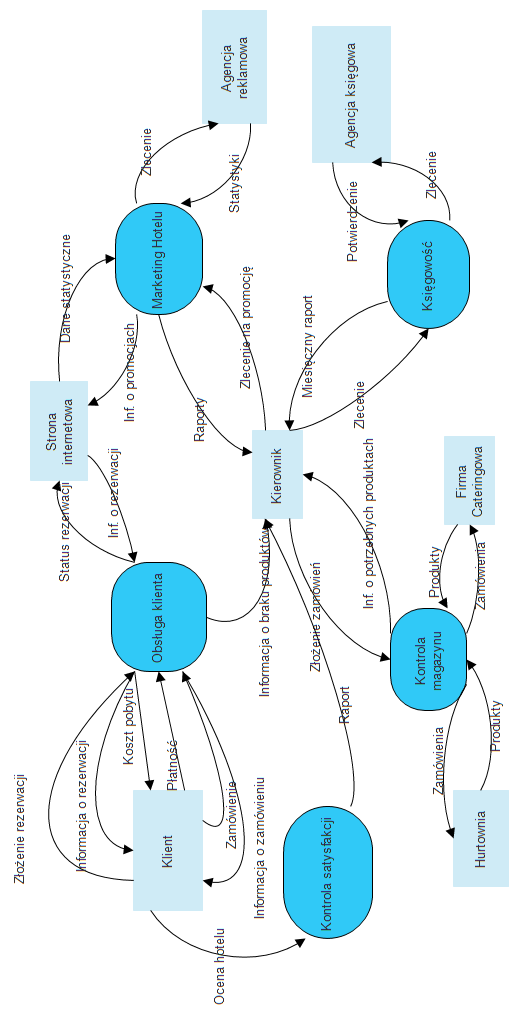
\includegraphics[scale=0.7]{Img/DFDpoziom0.png}
			\caption{Diagram DFD - proces 4.}
	\end{figure}
	\begin{figure}[H]%[!htb]
			\center
			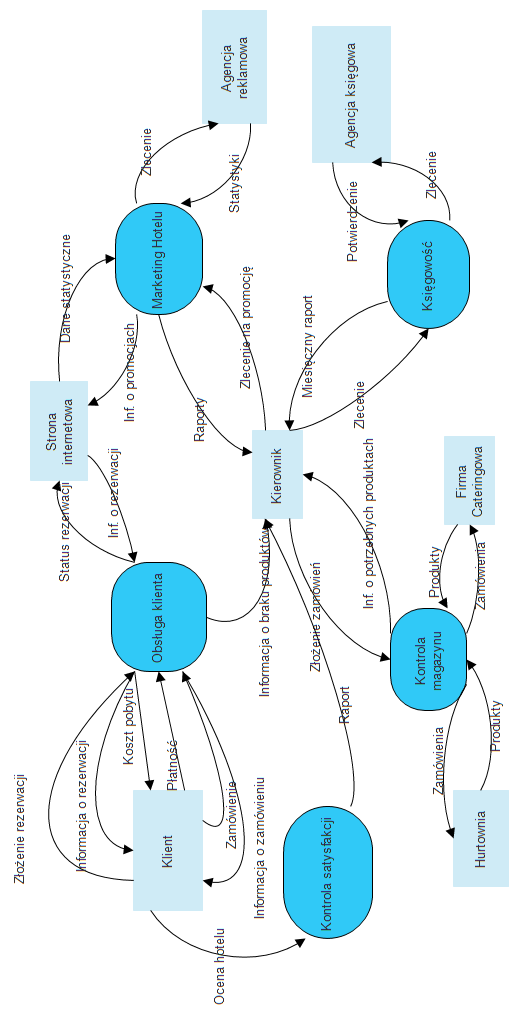
\includegraphics[scale=0.7]{Img/DFDpoziom0.png}
			\caption{Diagram DFD - proces 5.}
	\end{figure}


	\subsection{poziom 2}
	\indent
	\begin{figure}[H]%[!htb]
			\center
			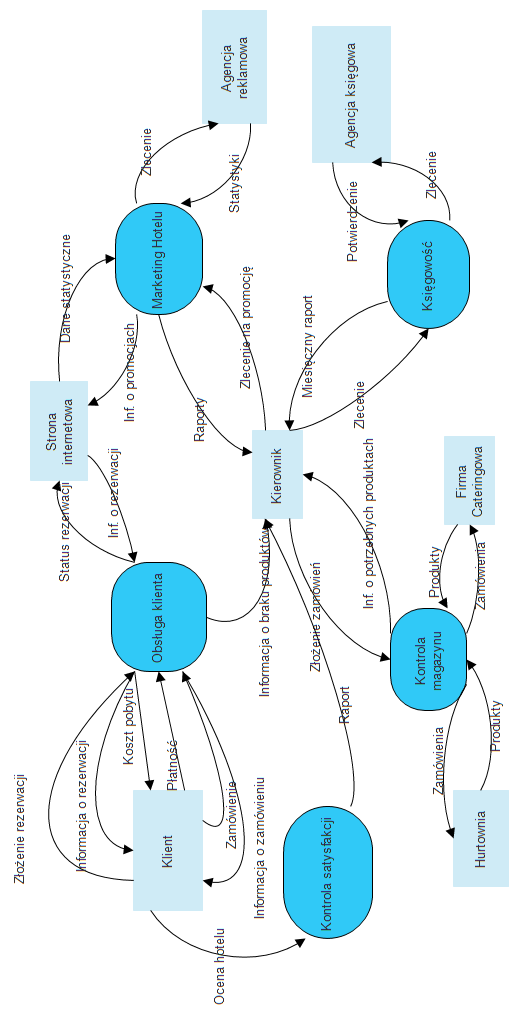
\includegraphics[scale=0.7]{Img/DFDpoziom0.png}
			\caption{Diagram DFD - proces 1.1}
	\end{figure}

	\begin{figure}[H]%[!htb]
			\center
			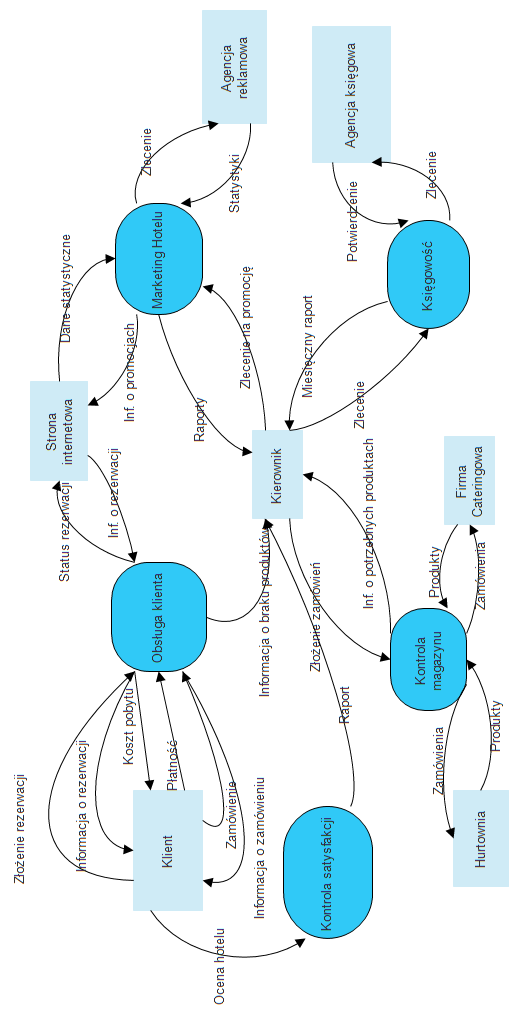
\includegraphics[scale=0.7]{Img/DFDpoziom0.png}
			\caption{Diagram DFD - proces 2.1}
	\end{figure}
	\begin{figure}[H]%[!htb]
			\center
			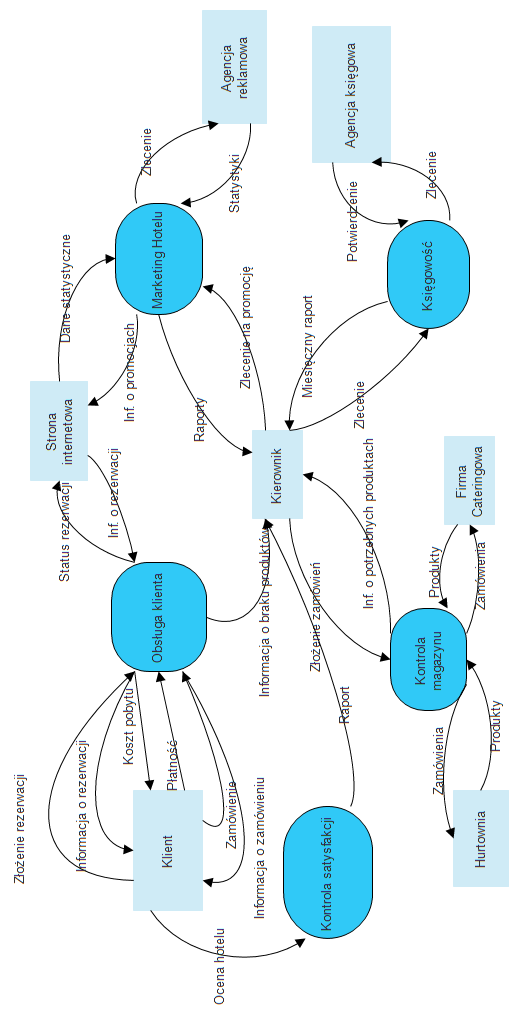
\includegraphics[scale=0.7]{Img/DFDpoziom0.png}
			\caption{Diagram DFD - proces 2.2}
	\end{figure}
	\begin{figure}[H]%[!htb]
			\center
			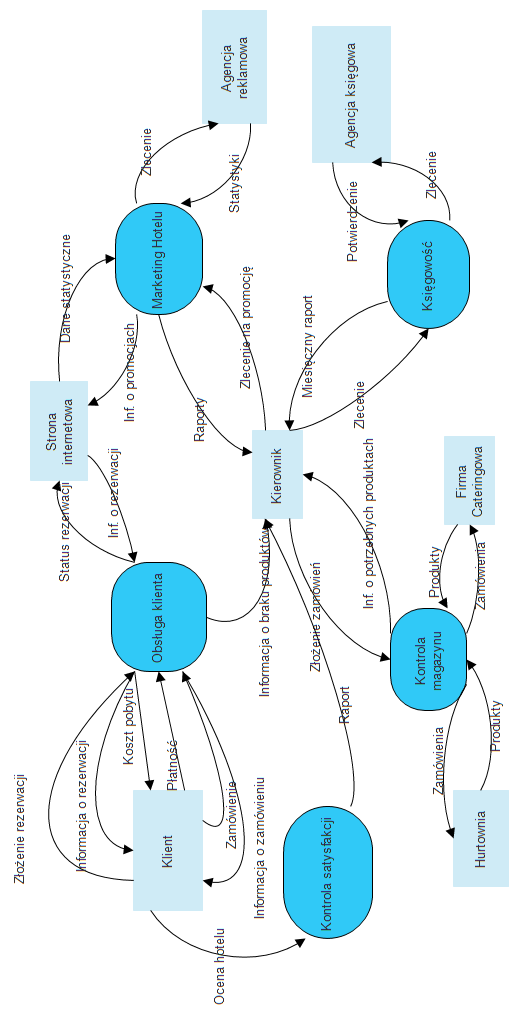
\includegraphics[scale=0.7]{Img/DFDpoziom0.png}
			\caption{Diagram DFD - proces 2.3}
	\end{figure}
	\begin{figure}[H]%[!htb]
			\center
			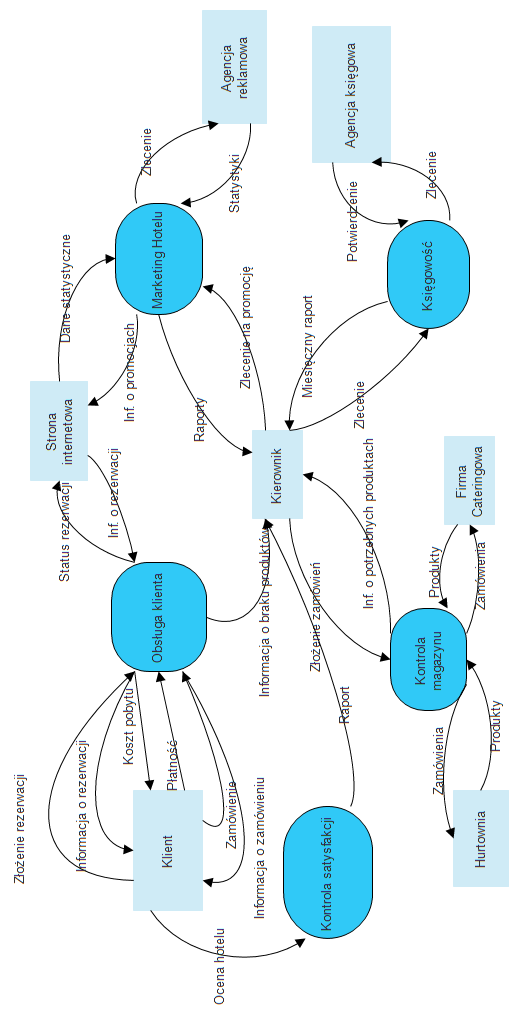
\includegraphics[scale=0.7]{Img/DFDpoziom0.png}
			\caption{Diagram DFD - proces 2.4}
	\end{figure}	
	\begin{figure}[H]%[!htb]
			\center
			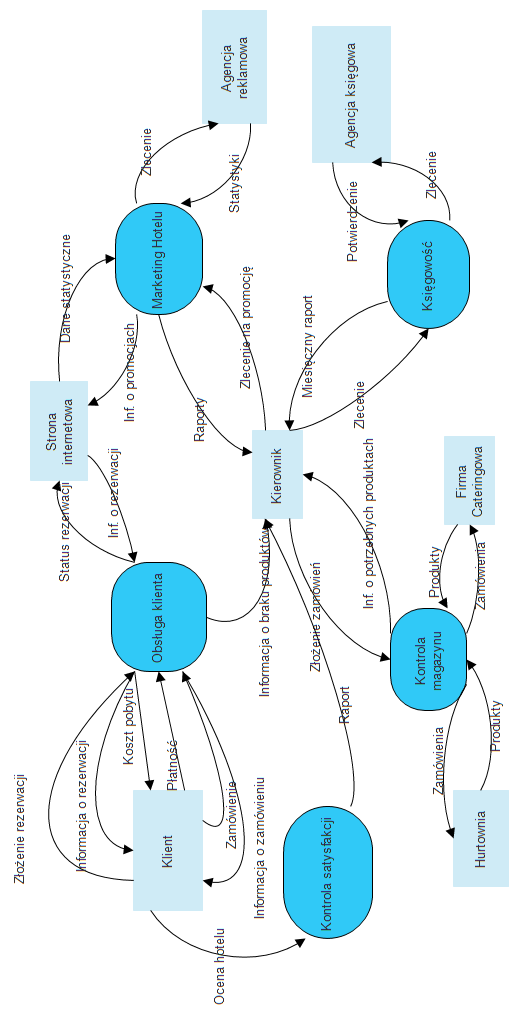
\includegraphics[scale=0.7]{Img/DFDpoziom0.png}
			\caption{Diagram DFD - proces 2.5}
	\end{figure}
	\begin{figure}[H]%[!htb]
			\center
			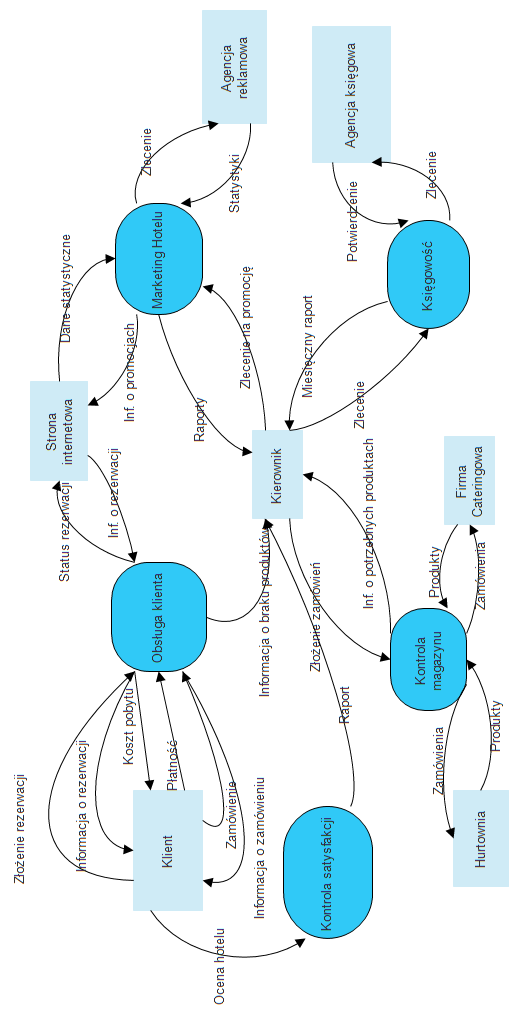
\includegraphics[scale=0.7]{Img/DFDpoziom0.png}
			\caption{Diagram DFD - proces 3.1}
	\end{figure}
	
		
	\subsection{poziom 3}
	\indent
	\begin{figure}[H]%[!htb]
			\center
			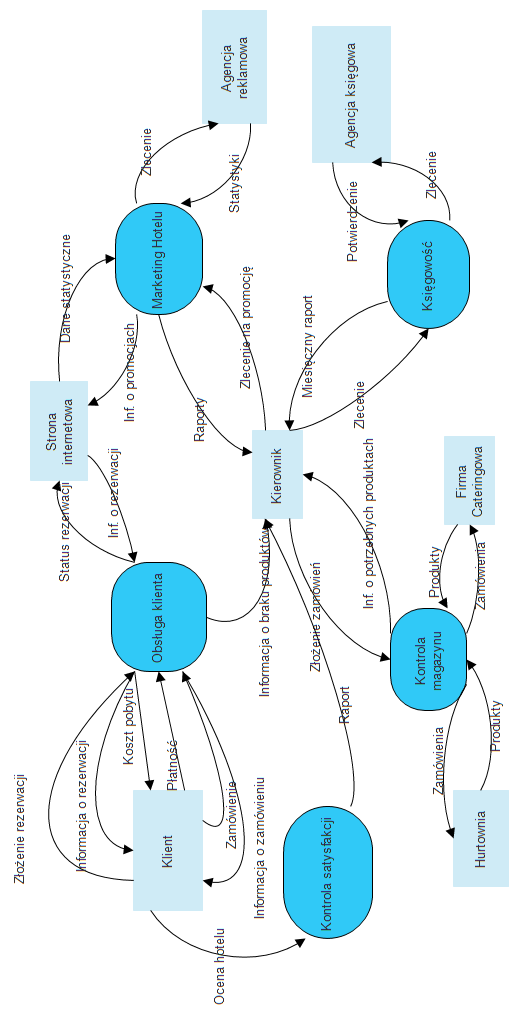
\includegraphics[scale=0.7]{Img/DFDpoziom0.png}
			\caption{Diagram DFD - proces 2.4.1}
	\end{figure}		
	
	
	
	
	
	\section{Diagram ERD}
	\indent
	\begin{figure}[H]%[!htb]
			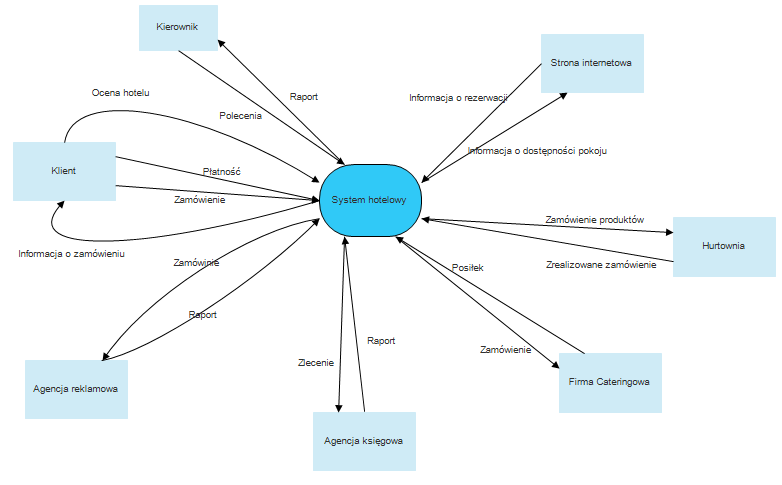
\includegraphics[scale=0.8]{Img/kontekstowy.png}
			\caption{Diagram kontekstowy}
	\end{figure}
	
	
	
	
	\newpage
	\section{Specyfikacja procesów PSPEC}
	\subsection{Spis}
		\begin{enumerate}[label*=\arabic*.]
		\item Kontrola satysfakcji
		\begin{enumerate}[label*=\arabic*.]
			\item Analiza ankiety
			\begin{enumerate}[label*=\arabic*.]
				\item Sprawdzenie poprawności ankiety
				\item Niszczenie ankiety
				\item Konwersja danych do postaci elektronicznej
			\end{enumerate}
			\item Stworzenie raportu, diagramów
		\end{enumerate}
		\item Obsługa klienta
		\begin{enumerate}[label*=\arabic*.]
			\item Obsługa rezerwacji
			\begin{enumerate}[label*=\arabic*.]
				\item Wcielenie rezerwacji
				\item Zdobywanie potrzebnych informacji
			\end{enumerate}
			\item Obsługa magazynu
			\begin{enumerate}[label*=\arabic*.]
				\item Przetworzenie danych
				\item Przetworzenie informacji
				\item Sumowanie kosztów zamówień
				\item Przygotowanie posiłku
			\end{enumerate}						
			\item Obsługa klienta meldującego się 
			\begin{enumerate}[label*=\arabic*.]
				\item Weryfikacja klienta
				\item Realizacja rezerwacji
				\item Powiadomienie klienta o stanie rezerwacji
			\end{enumerate}									
			\item Obsługa klienta wychodzącego
			\begin{enumerate}[label*=\arabic*.]
				\item Realizacja zapłaty
				\begin{enumerate}[label*=\arabic*.]
					\item Wybór sposobu płatności
					\item Uregulowanie kosztów
					\item Sporządzenie potwierdzenia
					\item Zliczenie kosztów
					\item Obciążenie konta
				\end{enumerate}													
				\item Składanie kluczy
				\item Wystawianie rachunku
				\item Zliczenie kosztów
			\end{enumerate}						
			\item Obsługa klienta przebywającego
			\begin{enumerate}[label*=\arabic*.]
				\item Rozdzielenie zamówień
				\item Przeniesienie bagażu
				\item Redakcja informacji o zamówieniach
				\item Zamówienie taksówki
				\item Zamówienie sprzątania
				\item Zamówienie posiłku
				\item Obsługa magazynu
			\end{enumerate}						
		\end{enumerate}
		\item Marketing hotelu
		\begin{enumerate}[label*=\arabic*.]
			\item Zarządzanie marketingiem
			\begin{enumerate}[label*=\arabic*.]
				\item Cykliczne wysyłanie zleceń
				\item Analiza raportów
			\end{enumerate}	
			\item Tworzenie raportu
		\end{enumerate}		
		\item Kontrola magazynu
		\begin{enumerate}[label*=\arabic*.]
			\item Rozdzielenie listy potrzeb
			\item Organizacja produktów z Hurtowni
			\item Organizacja produktów spożywczych
		\end{enumerate}	
		\item Księgowość
		\begin{enumerate}[label*=\arabic*.]
			\item Ustalenie priorytetów
			\item Tworzenie raportów
			\item Zbieranie potrzebnych dokumentów
		\end{enumerate}	
	\end{enumerate}

	
	


	\subsection{Opis}
	\begin{enumerate}[label*=\arabic*.]
		\item Kontrola satysfakcji
		\begin{enumerate}[label*=\arabic*.]
			\item Analiza ankiety
			\begin{enumerate}[label*=\arabic*.]
				\item Sprawdzenie poprawności ankiety
				\begin{description}
					\item[Wejście:]	Wypełniona ankieta 
					\item[Wyjście:]	Poprawna ankieta, Niepoprawna ankieta
					\item[Działanie:] Wypełnioną ankietę segreguje względem poprawności.
				\end{description}				
				\item Niszczenie ankiety
				\begin{description}
					\item[Wejście:] Niepoprawna ankieta
					\item[Wyjście:] 
					\item[Działanie:] Wrzucenie ankiety do niszczarki, wyrzucenie śmieci.
				\end{description}				
				\item Konwersja danych do postaci elektronicznej
				\begin{description}
					\item[Wejście:] Poprawna ankieta
					\item[Wyjście:] Elektroniczne wyniki ankiety
					\item[Działanie:] Przepisanie krok po kroku wszystkich pól z ankiety do systemu informatycznego i zapisanie wyników.
				\end{description}	
			\end{enumerate}
			\item Stworzenie raportu, diagramów
			\begin{description}
				\item[Wejście:] Ankiety w formie elektronicznej
				\item[Wyjście:] Raport wraz z diagramami
				\item[Działanie:] Wpierw sporządzenie na podstawie ankiet wykresów statystycznych zadowoleń. Następnie ich analiza i wyciągnięcie wniosków w postaci sprawozdania wraz z diagramami.
			\end{description}	
		\end{enumerate}
		\item Obsługa klienta
		\begin{enumerate}[label*=\arabic*.]
			\item Obsługa rezerwacji
			\begin{enumerate}[label*=\arabic*.]
				\item Wcielenie rezerwacji
				\begin{description}
					\item[Wejście:] Informacja o chęci rezerwacji, lista dostępnych pokoi, koszt noclegu
					\item[Wyjście:] dostępność pokojów i ich cena, stan rezerwacji klienta, sygnał żądania pobrania informacji o pokojach.
					\item[Działanie:] Przedstawienie w jasnej formie ofert pokoi i ich cen. Następnie zaakceptowanie wyboru klienta i przesłanie dalej informacji do aktualizacji bazy danych.
				\end{description}	
				\item Zdobywanie potrzebnych informacji
				\begin{description}
					\item[Wejście:] Informacje o dostępnych pokojach, żądanie o te informacje
					\item[Wyjście:] Informacje o dostępnych pokojach, żądanie o te informacje
					\item[Działanie:] Na żądanie informacji o dostępach pokoi, wysyła o nie zapytania do obsługi bazy danych, a jak już je uzyska, filtruje pokoje zajęte i przekazuje podmiotom zainteresowanym.
				\end{description}	
			\end{enumerate}
			\item Obsługa magazynu
			\begin{enumerate}[label*=\arabic*.]
				\item Przetworzenie danych
				\begin{description}
					\item[Wejście:] Żądanie informacji o rezerwacji, zmieniony stan rezerwacji
					\item[Wyjście:] Informacje o dostępnych pokojach
					\item[Działanie:] Na żądanie, pobiera informacje z bazy danych na temat rezerwacji. Następnie przetwarza je, do czytelniejszej postaci i odsyła zainteresowanemu podmiotowi. W przypadku otrzymania stanu rezerwacji, przekłada go na  system informatyczny i zapisuje dane.
				\end{description}	
				\item Przetworzenie informacji
				\begin{description}
					\item[Wejście:] Żądanie o dostępności pokoi
					\item[Wyjście:] Graficzna forma informacji o dostępnych pokoi
					\item[Działanie:] Na żądanie, pobiera informacje z bazy danych na temat dostępności pokoi. Następnie przetwarza je, do graficznej postaci i odsyła zainteresowanemu podmiotowi.
				\end{description}	
				\item Sumowanie kosztów zamówień
				\begin{description}
					\item[Wejście:] Koszty zamówień klienta, żądanie całkowitego kosztu
					\item[Wyjście:] Całkowity koszt klienta
					\item[Działanie:] Na żądanie, pobiera informacje z bazy danych na temat wszystkich usług i kosztów klienta. Następnie je sumuje i po przełożeniu do czytelniejszej formy, odsyła zainteresowanemu podmiotowi.
				\end{description}	
				\item Przygotowanie posiłku
				\begin{description}
					\item[Wejście:] nazwa posiłku
					\item[Wyjście:] posiłek
					\item[Działanie:] Na podstawie nazwy posiłku, pobiera składniki z magazynu produktów spożywczych, przygotowuje z nich zestaw, cały posiłek i wydaje dalej zainteresowanemu podmiotowi.
				\end{description}	
			\end{enumerate}						
			\item Obsługa klienta meldującego się 
			\begin{enumerate}[label*=\arabic*.]
				\item Weryfikacja klienta
				\begin{description}
					\item[Wejście:] Dane klienta
					\item[Wyjście:] Żądanie informacji dot. rezerwacji
					\item[Działanie:] Analizowanie danych osobowych klienta i sformułowanie poprawnego żądanie.
				\end{description}	
				\item Realizacja rezerwacji
				\begin{description}
					\item[Wejście:] Potwierdzenie istnienia rezerwacji, klucze
					\item[Wyjście:] Klucze, Stan rezerwacji
					\item[Działanie:] Na podstawie pozytywnej informacji o rezerwacji, dokonuje zmiany stanu rezerwacji na zrealizowana i stan ten propagowany jest dalej. Pobiera odpowiednie klucze z magazynu i udostępnia je klientowi.
				\end{description}	
				\item Powiadomienie klienta o stanie rezerwacji
				\begin{description}
					\item[Wejście:] Stan rezerwacji
					\item[Wyjście:]
					\item[Działanie:]
				\end{description}	
			\end{enumerate}									
			\item Obsługa klienta wychodzącego
			\begin{enumerate}[label*=\arabic*.]
				\item Realizacja zapłaty
				\begin{enumerate}[label*=\arabic*.]
					\item Wybór sposobu płatności
					\begin{description}
						\item Wejście: 
						\item Wyjście:
						\item Działanie: 
					\end{description}
					\item Uregulowanie kosztów
					\begin{description}
						\item Wejście: 
						\item Wyjście:
						\item Działanie: 
					\end{description}					
					\item Sporządzenie potwierdzenia
					\begin{description}
						\item Wejście: 
						\item Wyjście:
						\item Działanie: 
					\end{description}
					\item Zliczenie kosztów
					\begin{description}
						\item Wejście: 
						\item Wyjście:
						\item Działanie: 
					\end{description}
					\item Obciążenie konta
					\begin{description}
						\item Wejście: 
						\item Wyjście:
						\item Działanie: 
					\end{description}
				\end{enumerate}													
				\item Składanie kluczy
				\begin{description}
					\item Wejście: 
					\item Wyjście:
					\item Działanie: 
				\end{description}
				\item Wystawianie rachunku
				\begin{description}
					\item Wejście: 
					\item Wyjście:
					\item Działanie: 
				\end{description}
				\item Zliczenie kosztów
				\begin{description}
					\item Wejście: 
					\item Wyjście:
					\item Działanie: 
				\end{description}
			\end{enumerate}						
			\item Obsługa klienta przebywającego
			\begin{enumerate}[label*=\arabic*.]
				\item Rozdzielenie zamówień
				\begin{description}
					\item Wejście: 
					\item Wyjście:
					\item Działanie: 
				\end{description}
				\item Przeniesienie bagażu
				\begin{description}
					\item Wejście: 
					\item Wyjście:
					\item Działanie: 
				\end{description}
				\item Redakcja informacji o zamówieniach
				\begin{description}
					\item Wejście: 
					\item Wyjście:
					\item Działanie: 
				\end{description}
				\item Zamówienie taksówki
				\begin{description}
					\item Wejście: 
					\item Wyjście:
					\item Działanie: 
				\end{description}
				\item Zamówienie sprzątania
				\begin{description}
					\item Wejście: 
					\item Wyjście:
					\item Działanie: 
				\end{description}
				\item Zamówienie posiłku
				\begin{description}
					\item Wejście: 
					\item Wyjście:
					\item Działanie: 
				\end{description}
				\item Obsługa magazynu
				\begin{description}
					\item Wejście: 
					\item Wyjście:
					\item Działanie: 
				\end{description}
			\end{enumerate}						
		\end{enumerate}
		\item Marketing hotelu
		\begin{enumerate}[label*=\arabic*.]
			\item Zarządzanie marketingiem
			\begin{enumerate}[label*=\arabic*.]
				\item Cykliczne wysyłanie zleceń
				\begin{description}
					\item Wejście: 
					\item Wyjście:
					\item Działanie: 
				\end{description}
				\item Analiza raportów
				\begin{description}
					\item Wejście: 
					\item Wyjście:
					\item Działanie: 
				\end{description}
			\end{enumerate}	
			\item Tworzenie raportu
		\end{enumerate}		
		\item Kontrola magazynu
		\begin{enumerate}[label*=\arabic*.]
			\item Rozdzielenie listy potrzeb
			\begin{description}
				\item Wejście: 
				\item Wyjście:
				\item Działanie: 
			\end{description}
			\item Organizacja produktów z Hurtowni			
			\begin{description}
				\item Wejście: 
				\item Wyjście:
				\item Działanie: 
			\end{description}
			\item Organizacja produktów spożywczych
			\begin{description}
				\item Wejście: 
				\item Wyjście:
				\item Działanie: 
			\end{description}
		\end{enumerate}	
		\item Księgowość
		\begin{enumerate}[label*=\arabic*.]
			\item Ustalenie priorytetów
			\begin{description}
				\item Wejście: 
				\item Wyjście:
				\item Działanie: 
			\end{description}
			\item Tworzenie raportów
			\begin{description}
				\item Wejście: 
				\item Wyjście:
				\item Działanie: 
			\end{description}
			\item Zbieranie potrzebnych dokumentów			
			\begin{description}
				\item Wejście: 
				\item Wyjście:
				\item Działanie: 
			\end{description}
		\end{enumerate}	
	\end{enumerate}
	
	
	
	
		
\end{document}
